\graphicspath{{chapters/10/images/}}
\chapter{Least squares problems}

\section{Introduction}
Let $\{y_i\}_{i = 1, \dots, n}$ be the observed data and $m(t_i, \vec{\theta})_{i = 1, \dots, n}$ be the corresponding model prediction.
Then the objective function is defined as:

$$f(\vec{\theta}) = \frac{1}{2}\sum\limits_{j = 1}^nr_j(\vec{\theta}) = \frac{1}{2}||r(\vec{\theta})||_2^2$$

Where:

\begin{multicols}{2}
  \begin{itemize}
    \item $r_j(\vec{\theta}) = y_j-m(t_j \vec{\theta})$.
    \item $r(\vec{\theta}) = (r_1(\vec{\theta}), \dots, r_n(\vec{\theta}))^T$ is called the residual.
  \end{itemize}
\end{multicols}

In general the residual is a matrix such that:

$$r(\vec{\theta}) = [r_{ij}(\vec{\theta})]_{\substack{i = i, \dots, n\\j = 1, \dots, m}}$$

Where:

\begin{multicols}{2}
  \begin{itemize}
    \item $i$ iterates over $n$ residuals.
    \item $j$ iterates over $m$ observations.
  \end{itemize}
\end{multicols}

The matrix can be reshaped into a vector, considering a vector of residuals.
Defining:

$$J_k=J(\theta_k)\left[\frac{\partial r_I}{\partial\theta_i}\right]_{\substack{i=1, ...,n\\ I=1,...n}}$$

So that:

\begin{align*}
  f(\vec{\theta}) &= \frac{1}{2}||r(\vec{\theta})||_2^2 = \frac{1}{2}\sum\limits_{j=1}^nr_j^2(\vec{\theta})\\
  \nabla f(\vec{\theta}) &= \sum\limits_{j=1}^nr_j\nabla r_j(\vec{\theta}) = J(\vec{\theta})^Tr(\vec{\theta})\\
  \nabla^2 f(\vec{\theta}) &= J^T(\vec{\theta})J(\vec{\theta}) + \sum\limits_{j=1}^nr_j\nabla^2 r_j(\vec{\theta})
\end{align*}

Where $J^T(\vec{\theta})J(\vec{\theta})$ is easy to compute as it is known without new derivative computations and it can be used to approximate $\nabla^2f(\vec{\theta})$.

  \subsection{Linear problem}
  The linear problem is the simplest case.
  Consider to describe a variable $y = A_{\vec{\theta}}$, where $A$ is a matrix, $\vec{\theta}$ is the vector of parameters and $\bar{y}$ the observations.
  The residuals can be defined as:

  \begin{multicols}{2}
    \begin{itemize}
      \item $r(\vec{\theta})=A_{\vec{\theta}}-\bar{y}$.
      \item $f(\vec{\theta})= ||A_{\vec{\theta}}-\bar{y}||^2$.
      \item $\nabla f(\theta)=A^T(A_{\vec{\theta}}-\bar{y})$.
      \item $\nabla^2 f = A^TA$.
    \end{itemize}
  \end{multicols}

  If $f$ is convex then:

  $$\exists \theta^* \text{such that} \nabla f(\vec{\theta}^*)=0 \Leftrightarrow A^TA_{\vec{\theta}^*}=A^T\bar{y}$$

  Reaching a normal equation with a  linear system.

  \subsection{Non linear least squares problem}
  For non-linear least square problem the first approach is a modified line-search Newton method.
  The problem of quantifying the distance between model and data can be formalized as:

  $$f(\theta)= \frac{1}{2} \sum^m_{j=1} r_j^2 (\theta) \\ \nabla f(\theta) = J(\theta)^{T} r (\theta) \\ \nabla f(\theta) = J(\theta)^{T} J (\theta) + \sum^m_{j=1} r_j \theta \nabla^2 r_3 \theta$$

  The sum can be ignored as:

  \begin{multicols}{2}
    \begin{itemize}
      \item It contains second order derivatives, which are expensive to compute.
      \item The Newton direction is a quasi vector.
    \end{itemize}
  \end{multicols}

  At every iteration $k$ the approximated problem to be solved is:

  $$J(\theta_k)^TJ(\theta_k)p=-J(\theta_k)r(\theta_k) \\ J_k^TJ_kp=-J_k^T r_k$$

  This is a linear system that is solved as:

  $$f(\theta_k+p)= \frac{1}{2} ||r(\theta_k+p)||^2 \simeq \frac{1}{2} ||J_kp+r_k||^2$$

  This is the normal equation for a normal least squares problem.
  Under certain hypotheses the method converges quadratically.

    \subsubsection{Summary}
    Recalling that the Newton method is quadratic convergent, the matrix is not singular.
    The system should be solved starting with a problem in the form of sum of squares.
    Thanks to this, the problem can be rewritten in a simpler way and an approximation can be performed, leading to solving a linear system at each iteration.
    This approximation guides  rapidly to a solution.
    Linear search is being applied, by defining a direction and solving a new problem at each iteration.
    The biggest issue could be the non invertible matrix, but this can be solved.
    It should be noted that the approximation of the second order derivative could cause a over-estimation of the term.

\section{The Levenberg-Marquardt method}
The Levenberg-Markquardt method is a combination of the Gauss Newton with trust region.
At each iteration the problem to be solved is:

$$\min_{||p||\leq\delta_k} \frac{1}{2} ||J_kp-r_k||^2$$

A solution can be inside inside the trust region $\delta_k$ or on the border, which is not the minimum, but the smallest value that can be reached.
If a solution is inside the region is accepted.
Otherwise if $||p||\le\delta_k$ $p$ is a solution if and only if:

$$\exists\lambda \ge 0 \text{ such that } (J^TJ + \lambda I)p = -J^Tr$$

The general problem that needs to be solved is:

$$\begin{cases}(J^TJ + \lambda I)p = -J^Tr\\\lambda(\delta_k-||p||) = 0\end{cases}$$

\begin{multicols}{2}
  \begin{itemize}
    \item if $\beta$ is a solution and $||p||\leq\delta_k$ the algorithm ends.
    \item if $||p||=\delta_k$ , then $\bar{p}$ is a solution if and only if
      $\exists \lambda > 0$:

      $$(J^TJ-\lambda I)=-J^Tr \\ + \lambda(\delta_k-||p||)=0$$
  \end{itemize}
\end{multicols}
\noindent

If moving a bit from zero and the problem is still solved, this can be thought as a solution.
If the boundary is being hit: $\lambda(\delta_k-||p||)=0$, the matrix has to be moved a bit from the singularity.
The Levenberg-Marquardt is one of MATLAB default solvers and it converges quadratically when t is close to the solution, while if the residuals are big it does not perform well.

  \subsection{Bounds}
  The Lagrangian can be exploited for the equality constraint, but other boundaries can be had.
  Other approaches allow to not lose the approximation advantage.
  For example variable transformation can be applied.
  Some example of variable transformations are:

  \begin{align*}
    x \mapsto e^x\qquad&\qquad  \mathbb{R} \mapsto \mathbb{R}_0^+\\
    x \mapsto \frac{e^x}{1+e^x}\qquad&\qquad  \mathbb{R} \mapsto [0,1]\\
    x \mapsto a + (b-a)\frac{e^x}{1+e^x}\qquad&\qquad  \mathbb{R} \mapsto [a,b]\\
  \end{align*}

  Another solution could be to include the bound in the trust region.
  There is a need to check at every iteration if the bounds are being satisfied and the actual reduction.
  Evolutionary algorithms follow the evolution of the solution: at the beginning a solution is built a penalty for the boundaries is added.
  This is called in Matlab the trust region reflective and it is the default method when defining a problem with bounds.

  \subsection{Solving global minimum problem}
  This method has no guarantee to converge to the global minimum.
  To solve the global minimum problem a multi-start approach could be taken.
  In this approach the parameter optimization is started from different starting point and it is checked whether the same minimum is obtained.

\section{Gauss-Newton method}
The global optimization problem is solved with a multi-start approach, so the procedure is repeated with different starting point.
Let $N \in \mathbb{N}, \varepsilon > 0, J$ as defined before.
Select randomly $N$ vectors:

$\theta^1, \dots, \theta^n \in \mathbb{R}^n$

The multi start approach for Gauss-Newton method is outlined in algorithm \ref{algo:gauss-newton}.

\begin{algorithm}[H]
\DontPrintSemicolon
\SetKwComment{comment}{$\%$}{}
\SetKw{Int}{int}
\SetKw{To}{to}
\SetKw{Return}{return}
\SetKw{Not}{not}
\SetKw{Input}{Input}
\SetKw{Output}{Output}
\SetKw{False}{false}
\SetKw{True}{true}
\SetKwData{Item}{item}
\SetKwFunction{Min}{min}
\SetKwFunction{Partitioning}{partitioning}
\SetKwFunction{TitleFunction}{Multi start approach for Gauss-Newton}

\caption{\protect\TitleFunction{}}
\label{algo:gauss-newton}

\Input: the Jacobian $J$ and the $N$ vectors of $\theta$\;

\Output: the optimal vector $\Theta$\;

\ForEach{$i = 1,\dots,N$}{
	\Repeat{$\epsilon<\delta$}{
		compute $q$ such that $\bar{J}^i\bar{J}q = -\bar{J}r(\theta^i)$\;
		$\vartheta = \theta^i+q$\;
		$\epsilon = \biggr\vert\biggr\vert \frac{\theta^-\vartheta}{\theta}\biggr\vert\biggr\vert $, the relative increase or $\epsilon = ||\bar{J}(\vartheta)$\;
		$\theta^i = \vartheta$\;
	}
	store $\theta_i$\;
}
\Return $\theta_i$ such that $r(\theta^i = \min\{||r(\theta^1)||, \dots, ||r(\theta^N)\})$\;

\end{algorithm}


This algorithm does not guarantee that the global minimum is obtained.

  \subsection{Determining the initial points}
  Randomly selecting the points may lead to have cluster of points and parts of the space not considered, which could lead to unsuccessful optimization.
  To better spread the points two strategies can be applied.

    \subsubsection{Latin hypercube}
    The Latin hypercube divides the space in equiprobable intervals or subspaces.
    It assures that for each interval row and column there is only one point selected.
    This is the most used method.

    \subsubsection{Orthogonal cube}
    The orthogonal cube divides the space in a equi-probable sub spaces and inside each sub space there are equally dense points.
    The total set of points is a Latin hypercube.

  \subsection{Termination criteria}
  Different termination criteria could be employed.

  \begin{itemize}
    \item Gradient equal to zero:

      $$||\nabla f||= 0\qquad\lor\qquad ||\nabla f||<\epsilon$$

    \item Relative step size:

      $$\biggr\vert\biggr\vert\frac{\theta^i-\vartheta}{\theta^i}\biggr\vert\biggr\vert<\epsilon$$

    \item Relative function change:

      $$\biggr\vert\biggr\vert\frac{f(\theta^i)-f(\vartheta)}{f(\theta^i)}\biggr\vert\biggr\vert<\epsilon$$

    \item Maximum number of iterations.
    \item Maximum number of function evaluations.
  \end{itemize}

\section{Matlab}
In Matlab, when an optimizer stops, it gives as output the function converged to the solution or why it stopped.
Termination criteria are:

\begin{multicols}{2}
  \begin{itemize}
    \item Gradient.
    \item Incremental step: if the change was less than a tolerance the residual is less.
    \item Number of iteration.
  \end{itemize}
\end{multicols}

According to different starting points, different results will be obtained.

  \subsection{Quantifying the fit}
  To quantify how much the model is distant from the real data consider the output of the normal simulation: this is a set of points,
  A linear interpolation for time and values can be performed, giving how much is each of the simulated variables at the requested time.
  Once the values at the right time are computed, the residuals can be calculated from the sum of squares.

  \subsection{Optimizing}
  To optimize in Matlab the function \texttt{lsqnonlin} can be used to improve the initial conditions.

  \subsection{Matlab multi-start}
  Matlab multi-start is a wrapper working with different algorithms.
  It will automatically parallelize the problem.
  It requires to insert starting points and tolerance.
  Then the bounds are defined, the problem is created and the initial input is given as input.
  The output contains the result of parallel lsqnonlin and parameters, somehow similar to what we saw before.
  The bounds can be reduced, but solution 1 of figure \ref{fig:lsqnonlin} is still the best.
  The main limitation is that this algorithm heavily depends on the initial points.

  \begin{figure}[H]
    \centering
    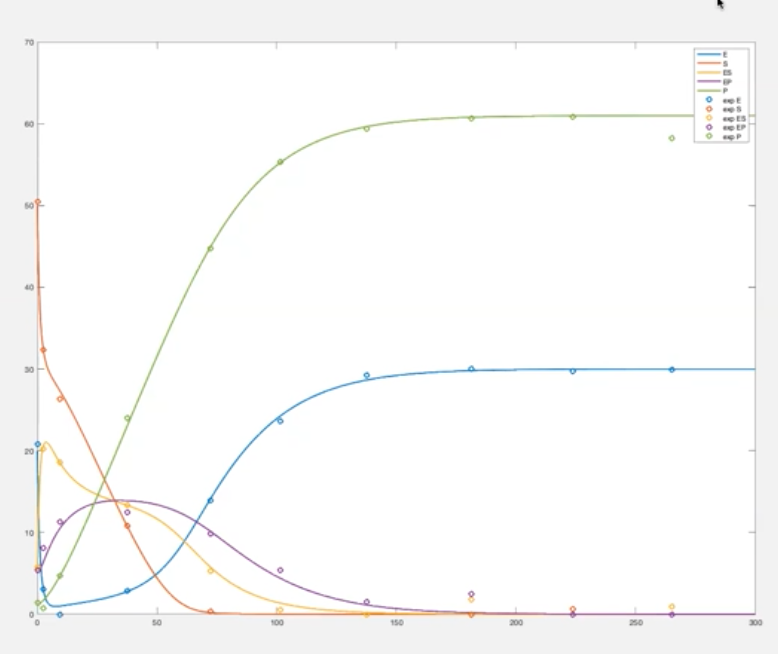
\includegraphics[width=0.45\textwidth]{multistep.png}
    \caption{MATLAB multi-start lsqnonlin}
    \label{fig:lsqnonlin}
  \end{figure}
